\documentclass{article}[]
\usepackage{epsfig}
\usepackage{psfig}
\usepackage{graphicx}
\usepackage{url}
\usepackage{tikz}
\usetikzlibrary{matrix,chains,positioning,decorations.pathreplacing,arrows}
\begin{document}

\title{{\bf Credit risk prediction using Artificial Neural Network algorithm}\\ }

\author{Shruti Goyal\\ \vspace{0.4cm}\\ 
 16200726 \vspace{0.1cm}\\ MSc Business Analytics \vspace{0.1cm}\\ 
 UCD Michael Smurfit Graduate Business School}

\date{}
\maketitle
\begin{abstract}
  Artificial neural network is an information processing system which is influenced by human brain and works on the same principles of biological nervous system. They possess ability to extract meaning from complex and intricate data, by detecting trends and extracting patterns from it. This paper illustrates the ability of neural network model constructed to predict the creditworthiness of an application accurately and precisely with minimal false predictions and errors. The results are shown to be robust, validated by scaling the dataset and compared with logistic regression model. \\ \\
  \textbf{Keywords:} Credit Risk, Artificial Neural Network, Prediction
\end{abstract}

\section{Introduction}
\label{intro}
Credit risk or credit default indicates the probability of non-repayment of bank financial services that has been given to the customers. Credit risk has always been an extensively studied area in bank lending decisions. Credit risk plays a crucial role for banks and financial institutions, especially for commercial banks and it is always difficult to interpret and manage. Due to the advancements in technology, banks have managed to reduce the costs, in order to develop robust and sophisticated systems and models to predict and manage credit risk.
The objective of credit risk models is to evaluate the risk portfolio of the borrower and then assign a probability of default. Therefore, there has been a discussion on classification and discrimination problems for solving credit risk models \cite{pacelli2011artificial}. \\\\
Banks evaluate loan applications based on a subjective assessment made by the borrower. This assessment can lead to inefficient and inconsistent applications. Banks will be successful if they are able to reduce the credit risk and have a significant effect on economic growth of the country. In order to discriminate between good customers and bad customers, banks developed a need for a model-based approach that can predict credit default accurately. The model-based approach provides better credit default management and efficiently allocate capital \cite{angelini2008neural}. \\\\
To predict the credit default, several methods have been created and proposed. The use of method depends on the complexity of banks and financial instituions, size and type of the loan. The commonly used method has been discrimination analysis. This method uses a score function that helps in decision making whereas some researchers have stated doubts on the validity of discriminates analysis because of its restrictive assumptions; normality and independence among variables \cite{eisenbeis1977pitfalls}. Artificial neural network models have created to overcome the shortcomings of other inefficient credit default models.\\\\
The objective of this paper is to study the ability of neural network algorithms to tackle the problem of predicting credit default, that measures the creditworthiness of the loan application over a time period. Feed forward neural network algorithm is applied to a small dataset of residential mortgages applications of a bank to predict the credit default. The output of the model will generate a binary value that can be used as a classifier that will help banks to identify whether the borrower will default or not default. This paper will follow an empirical approach which will discuss two neural network based models and experimental results will be reported by training and validating the models on residential mortgage loan applications. As the final step in the direction, logistic regression method is also performed on the dataset. Results will provide a comparison between the efficiency and accuracy of the neural network and logistic regression methods. As the paper follows an empirical approach, this paper will show structured experimental approach to the design of models. 

\section{Artificial Neural Network}
Discriminant analysis method has been the most common method to build credit default or credit score models. Although, this linear methodology has been criticized by the researchers because of its assumptions on the categorical data and unequal covariance matrices of good and bad customer loans.\\\\
An artificial neural network is a nonlinear approach that provides a new alternative to linear methods, especially in the situations where the dataset possess complex relationships between the independence of the nonlinear variables \cite{atiya2001bankruptcy} \cite{pang2002credit}. Artificial neural network is a learning system that models a relationship between inputs and outputs, taking into account the relationship is nonlinear. They are also known as black box systems, in which extraction of information from internal system is impossible \cite{angelini2008neural}.\\\\
Artificial Neural networks are machine learning system that simulates structure and function similar to a biological neuron. ANNs perform a task by changing its parameters, the same way a neuron changes its states to perform a cognitive task. A network is composed of a set of neurons structured in a specified topology. Neurons are connected by links with associated weights which determines information flow intensity; weights are the functions that represent behavior of the neural network.\\\\
\begin{figure}
\centering
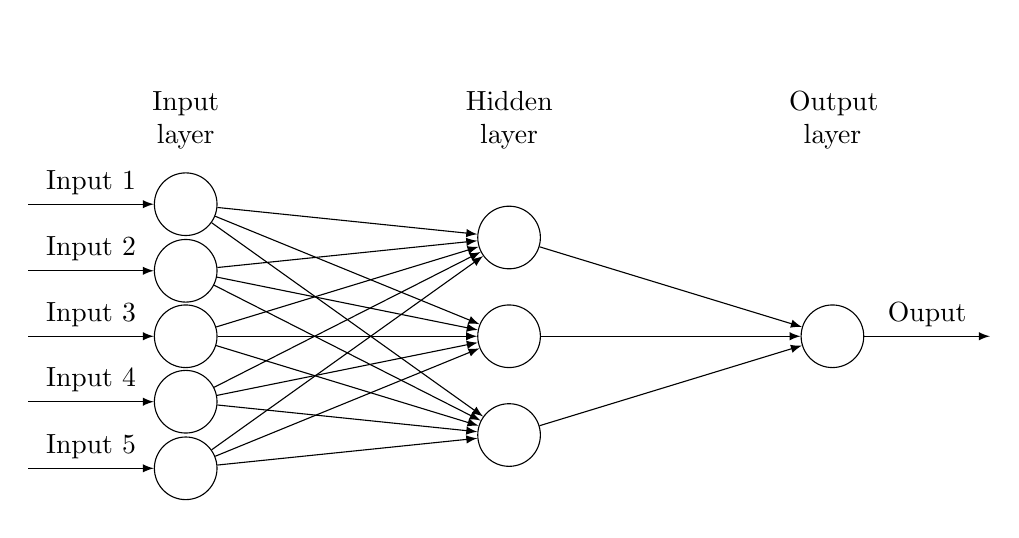
\begin{tikzpicture}[
plain/.style={
  draw=none,
  fill=none,
  },
net/.style={
  matrix of nodes,
  nodes={
    draw,
    circle,
    inner sep=8pt
    },
  nodes in empty cells,
  column sep=2cm,
  row sep=-11pt
  },
>=latex
]
\matrix[net] (mat)
{
|[plain]| \parbox{1.1cm}{\centering Input\\layer} & |[plain]| \parbox{1.1cm}{\centering Hidden\\layer} & |[plain]| \parbox{1.1cm}{\centering Output\\layer} \\
& |[plain]| \\
|[plain]| & \\
& |[plain]| \\
  |[plain]| & |[plain]| \\
& & \\
  |[plain]| & |[plain]| \\
& |[plain]| \\
  |[plain]| & \\
& |[plain]| \\    };
\foreach \ai [count=\mi ]in {2,4,...,10}
  \draw[<-] (mat-\ai-1) -- node[above] {Input \mi} +(-2cm,0);
\foreach \ai in {2,4,...,10}
{\foreach \aii in {3,6,9}
  \draw[->] (mat-\ai-1) -- (mat-\aii-2);
}
\foreach \ai in {3,6,9}
  \draw[->] (mat-\ai-2) -- (mat-6-3);
\draw[->] (mat-6-3) -- node[above] {Ouput} +(2cm,0);
\end{tikzpicture}
\caption{Basic Structure of Artificial Neural Network}
\label{fig:ANN1}
\end{figure}
As shown in figure \ref{fig:ANN1}, ANN has three layers, input layer, a hidden layer and output layer, input layer represents neurons receiving input stimulus. Then the information is transferred to next level of layer known as a hidden layer. Information is weighed before sending to next level of layers depending upon the size of the connections amongst neurons. Information is sized as per the processing unit or a transfer function represented in figure \ref{fig:ANN2}.\\
\begin{figure}
\centering
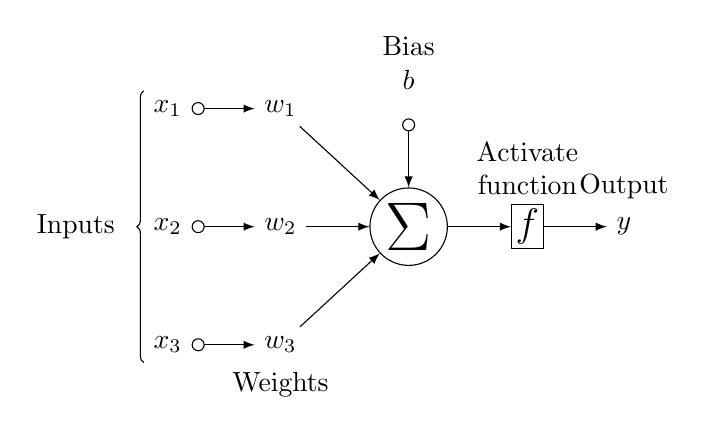
\begin{tikzpicture}[
init/.style={
  draw,
  circle,
  inner sep=1.5pt,
  font=\Huge,
  join = by -latex
},
squa/.style={
  draw,
  inner sep=1.5pt,
  font=\Large,
  join = by -latex
},
start chain=2,node distance=8mm
]
\node[on chain=2] 
  (x2) {$x_2$};
\node[on chain=2,join=by o-latex] 
  {$w_2$};
\node[on chain=2,init] (sigma) 
  {$\displaystyle\Sigma$};
\node[on chain=2,squa,label=above:{\parbox{1.5cm}{\centering Activate \\ function}}]   
  {$f$};
\node[on chain=2,label=above:Output,join=by -latex] 
  {$y$};
\begin{scope}[start chain=1]
\node[on chain=1] at (0,1.5cm) 
  (x1) {$x_1$};
\node[on chain=1,join=by o-latex] 
  (w1) {$w_1$};
\end{scope}
\begin{scope}[start chain=3]
\node[on chain=3] at (0,-1.5cm) 
  (x3) {$x_3$};
\node[on chain=3,label=below:Weights,join=by o-latex] 
  (w3) {$w_3$};
\end{scope}
\node[label=above:\parbox{2cm}{\centering Bias \\ $b$}] at (sigma|-w1) (b) {};

\draw[-latex] (w1) -- (sigma);
\draw[-latex] (w3) -- (sigma);
\draw[o-latex] (b) -- (sigma);

\draw[decorate,decoration={brace,mirror}] (x1.north west) -- node[left=7pt] {Inputs} (x3.south west);
\end{tikzpicture}
\caption{Mathematical Equation of Artificial Neural Network}
\label{fig:ANN2}
\end{figure}
Each neuron is characterized by a minimum value that activates a neuron(threshold value) and a transfer function. A Hidden layer can consist of several layers and performs the summation of input neurons and multiplies the weights with the summation to generate output neurons. Output generation is a two-step process: first, each input is multiplied by the weight on corresponding connection and then all valued are summed together; second, activation function is applied to summation of the inputs \cite{angelini2008neural}.\\
\begin{equation}
y_{i} = \sum_{j \in I} W_{j,i}a_{j}
\label{eq:1}
\end{equation}

\begin{equation}
a_{i} = g(y)    
\label{eq:2}
\end{equation}

Equation \ref{eq:1} represents evaluation of input and \ref{eq:2} represents activation function; where $W_{j,i}$ represents weights on the connection between $j$ and $i$ and $a_{j}$ is activation function of neuron $j$.\\\\
For a neural network to work efficiently, weights should be tuned accurately. This task can be achieved by using a learning algorithm, which trains the network and modifies weights until verified. Mostly, these algorithms stop when there occurs an error between output generated by network falls under threshold and expected output. There are three types of learning algorithms for artificial neural networks \cite{angelini2008neural}:
\begin{enumerate}
\item Supervised Learning
\item Unsupervised Learning
\item Reinforced Learning
\end{enumerate}

In supervised learning, a training set of correct examples is being used to train the network model. It consists of pairs of several inputs and expected outputs. Weights will be tuned based on the errors generated in the network. Most common example of supervised learning is classification, where the network has to learn to generalize relations between corresponding input and output variables. In this paper, we will be dealing with the typical classification problem to predict the credit default. 

\section{Methodology}
\bibliographystyle{abbrv}
\bibliography{biblio} 

\end{document}

